% Author : Alain Matthes
% Encoding : UTF8
% Engine : PDFLaTeX
\documentclass[]{article}
\usepackage[utf8]{inputenc} 
\usepackage[usenames,dvipsnames]{xcolor}
\usepackage{fullpage}
\usepackage[upright]{fourier}
\usepackage{tkz-berge}
\thispagestyle{empty}

\begin{document}
	
\tikzstyle{VertexStyle}=[shape         = circle,%
                         fill          = red!50,
                         very thin,
                         inner sep    = 0pt,%
                         minimum size = 16pt,
                         draw]
\tikzstyle{EdgeStyle}= [thick,%
                        double= lightgray,%
                        double distance = 1pt]

  \SetVertexLabel
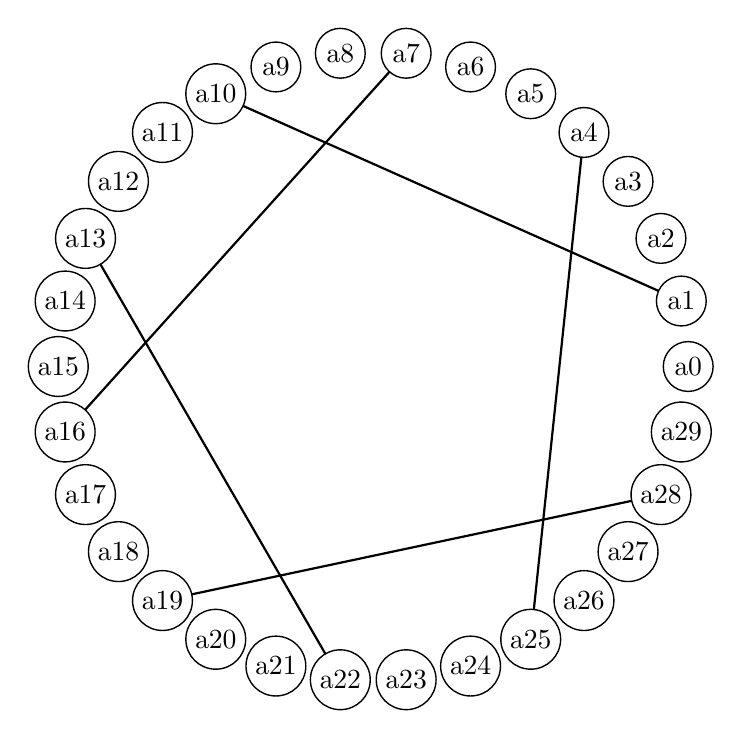
\begin{tikzpicture}
         \grEmptyCycle[RA=4]{30}
         \EdgeInGraphMod*{a}{30}{9}{1}{6} 
\end{tikzpicture}

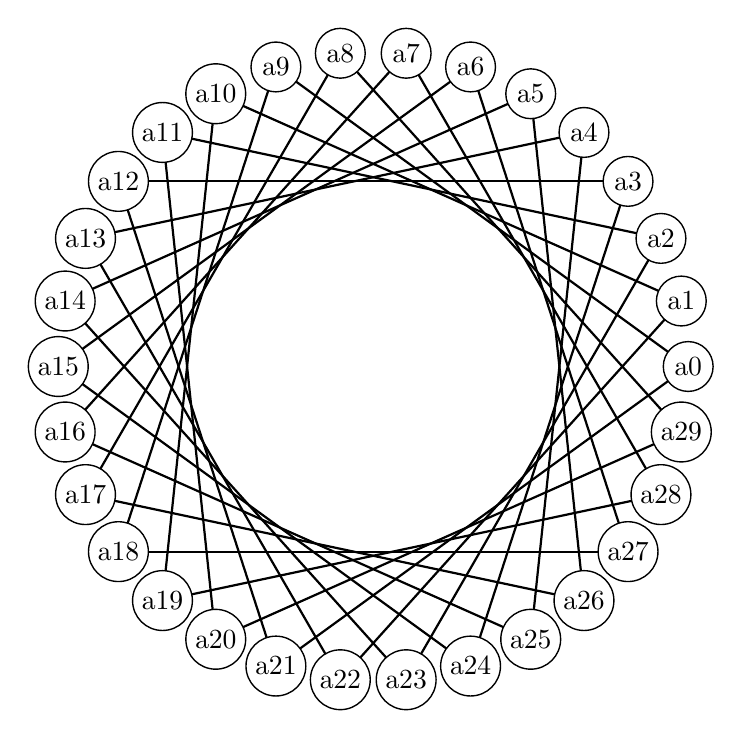
\begin{tikzpicture}
         \grEmptyCycle[RA=4]{30}
        \EdgeInGraphMod{a}{30}{9}
\end{tikzpicture}

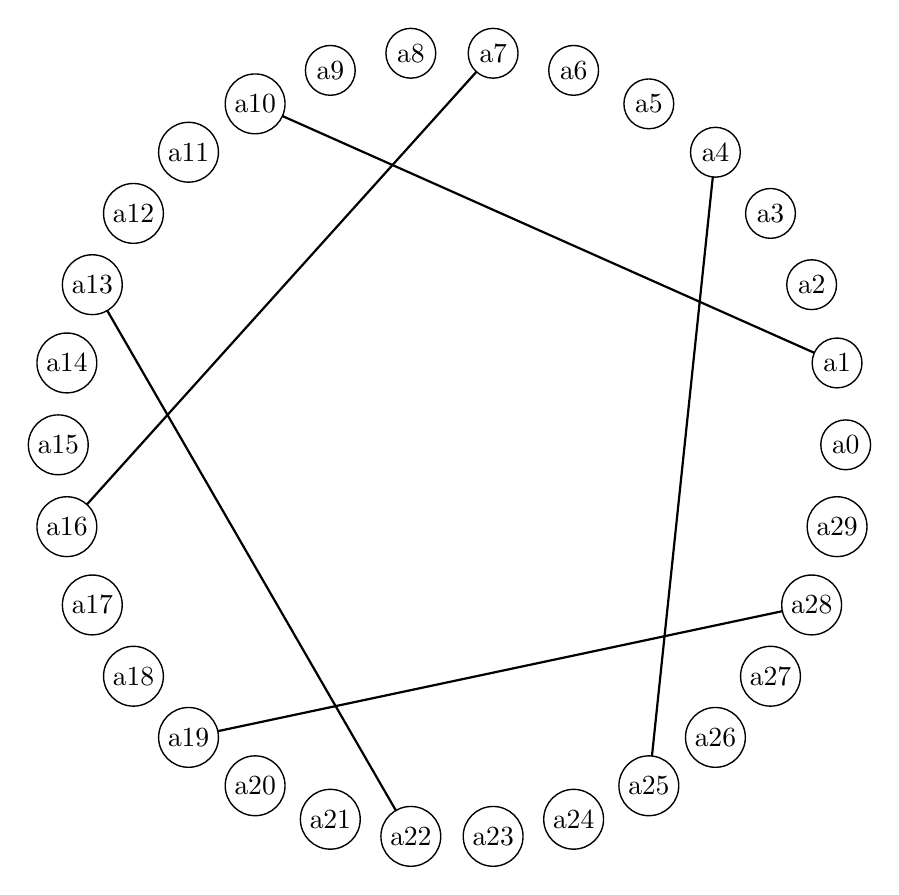
\begin{tikzpicture}
         \grEmptyCycle[RA=5]{30}
        \EdgeInGraphMod*{a}{30}{9}{1}{6}
\end{tikzpicture}

\begin{center}
 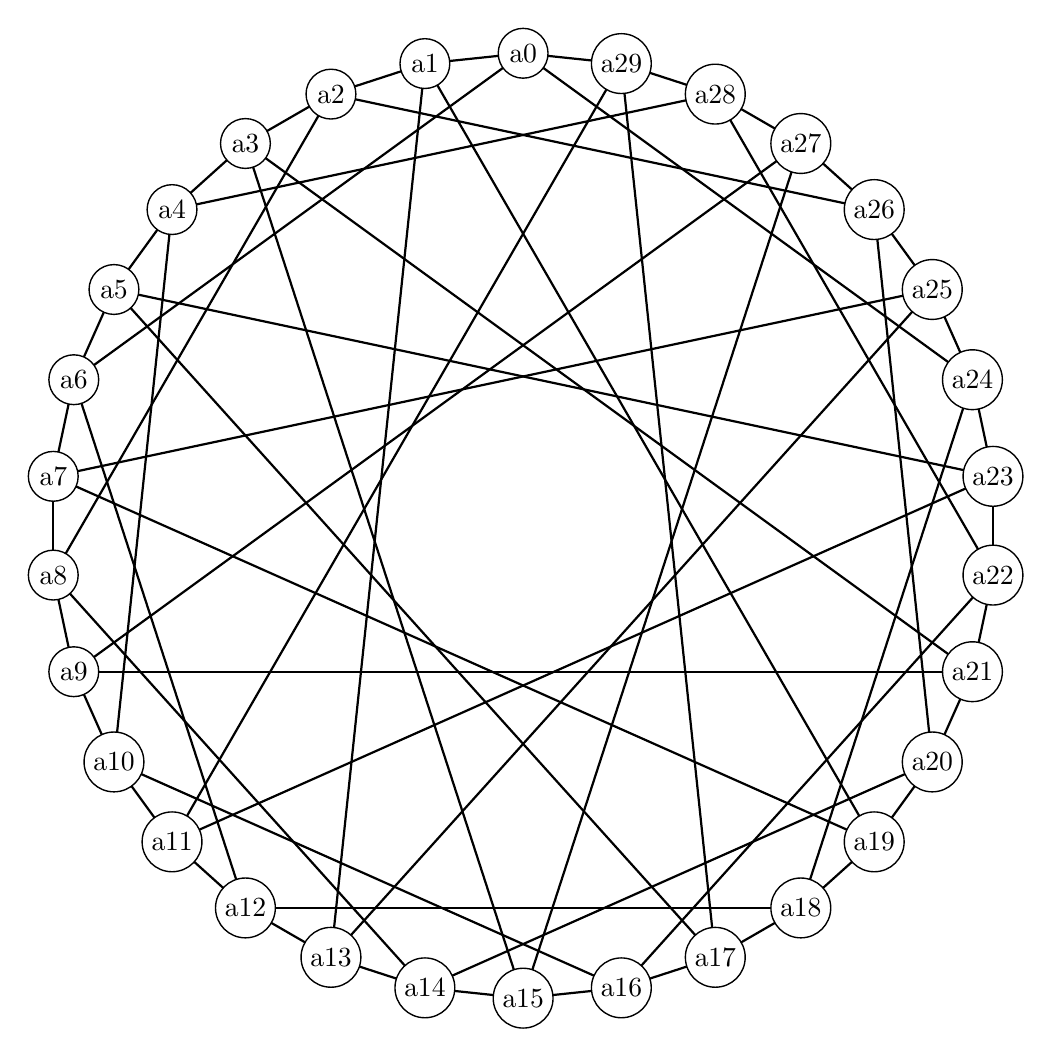
\begin{tikzpicture}[rotate=90]
   \grLCF[RA=6]{6,12}{15}
  \end{tikzpicture}
\end{center}


\begin{center}
 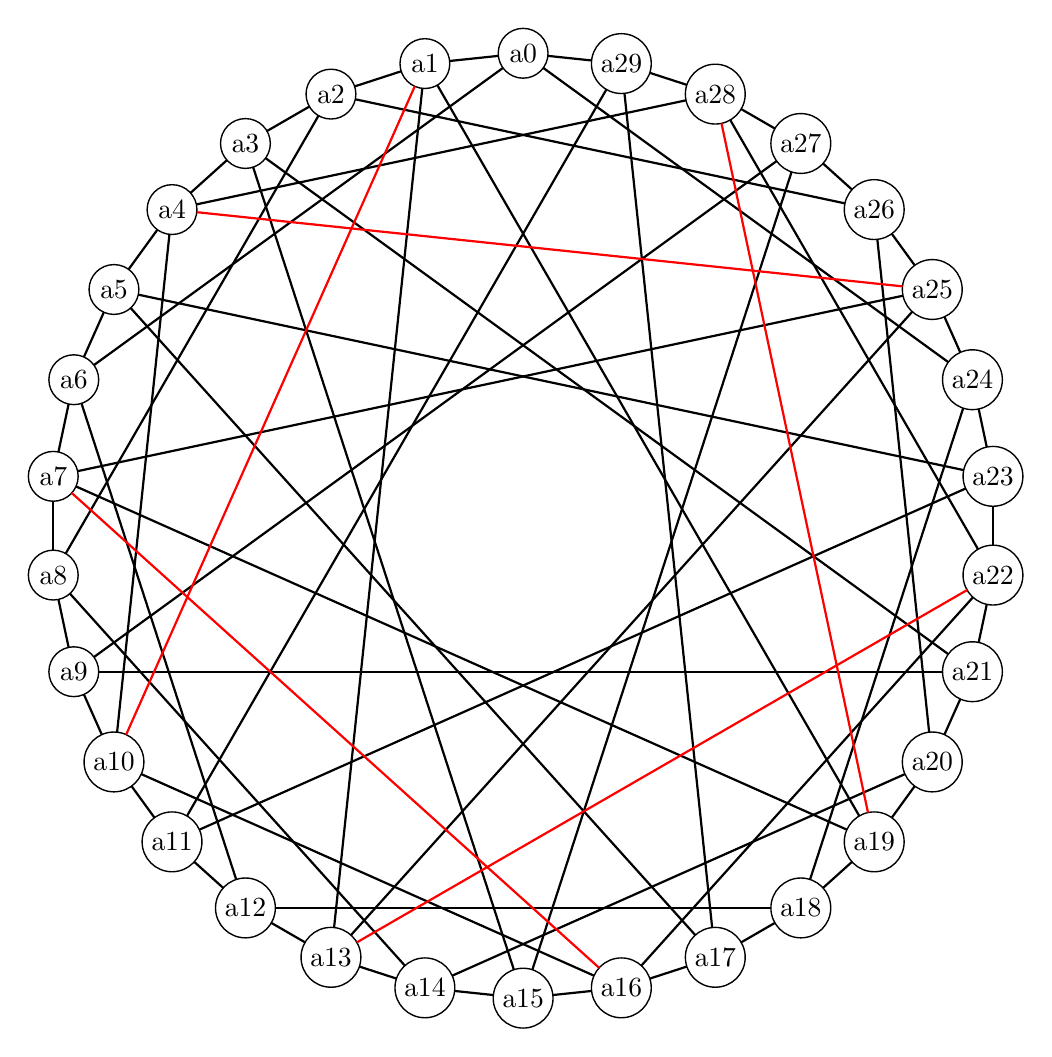
\begin{tikzpicture}[rotate=90]
   \grLCF[RA=6]{6,12}{15}
   \SetUpEdge[color=red]
   \EdgeInGraphMod*{a}{30}{9}{1}{6}
  \end{tikzpicture}
\end{center}

\begin{center}
 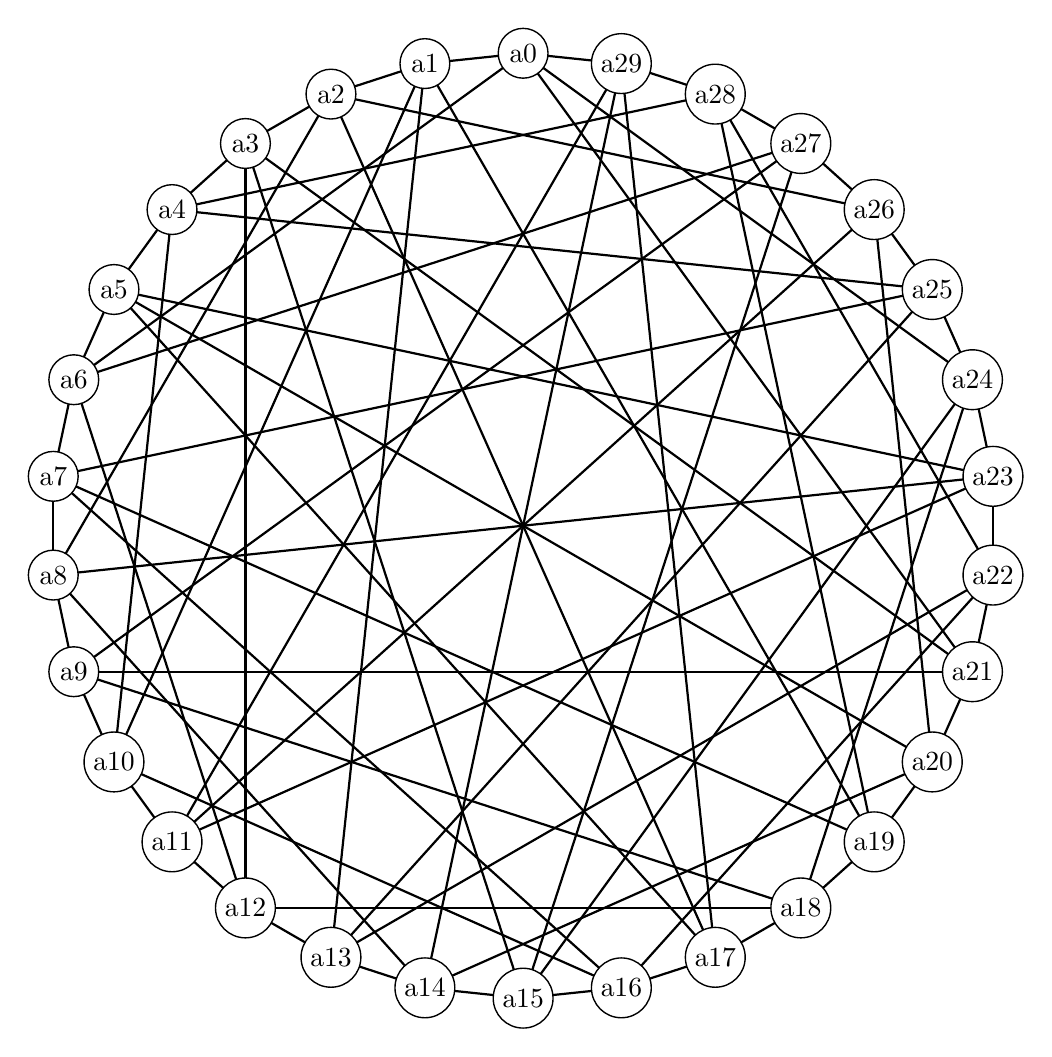
\begin{tikzpicture}[rotate=90]
   \grLCF[RA=6]{6,12}{15}
   \EdgeInGraphMod*{a}{30}{9}{1}{6}
   \EdgeInGraphMod*{a}{30}{15}{2}{6}
   \EdgeInGraphMod*{a}{30}{9}{3}{6}
  \end{tikzpicture}
\end{center}

\end{document}
